\documentclass[10]{article}

\usepackage{ctex}
\usepackage{graphicx}
\usepackage {subfigure}
\usepackage{float}
\usepackage{amsmath}
\usepackage{amssymb}

\bibliographystyle{plain}
\title{Regression}
\author{Prevalenter}
\date{\today}

\begin{document}
	\maketitle
	\section{简介}
	本文主要介绍了李宏毅老师的机器学习课程中的Demo1的例子,对Gradient Descent与Adagrad进行了简单的公式介绍,并对两种方式进行了编程仿真,其仿真源码对于代码文件的Regrassion中。
	\section{公式推导}
		\subsection{定义模型}
			李宏毅老师在课程中定义的模型为线性的,如公式\ref{e1}所示,其中w代表权重,b代表偏置值,x代表输入值,y代表输出值。
			\begin{gather}
				y=b+w*x\label{e1}
			\end{gather}
			当写出矩阵的形式,如公式\ref{e2}所示。
%				y=b+w*x\label{e1}
			\begin{gather}
				y=\begin{pmatrix}
				w & b
				\end{pmatrix}
				\begin{pmatrix}
				x\\
				1\\
				\end{pmatrix}\label{e2}
			\end{gather}

		\subsection{定义损失函数}
		直接通过计算预测得到的直线与标记后的数据的距离,来定义损失函数,公式如\ref{e3}所示。
			\begin{equation}
				\begin{split}
				\ L(f)&=L(w,b) \\
				&=\sum_{n=1}^{10}(\hat{y}-(b+w*x^{n}))^{2}\label{e3}
				\end{split}
			\end{equation}
		\subsection{迭代方法}
			当我们通过公式定义了模型,通过公式定义了损失函数后,实际上就可以通过迭代的方法寻找$ f^{*} $,即$ w^{*} $与$ b^{*} $,可用公式表达。
			\begin{gather}
				f^{*}=\arg \min(f)	\label{e4}
			\end{gather}		
			\begin{equation}
				\begin{split}
				\ w^{*},b^{*}&=\arg \min_{w,b}L(w,b) \\
				&=\arg \min_{w,b}(\hat{y}-(b+w*x^{n}))^{2}\label{e5}
				\end{split}
			\end{equation}
			但是选择正确迭代方法,对于能否找到合适的w与b值是至关重要的,视频中介绍的方法主要有Gradient Descent与Adagrad两种方法。
			\subsubsection{Gradient Descent}
			Gradient Descent又称梯度下降,是最基础的一种迭代方法。其大致思路为:随机或人工设定$ w $与$ b $的初始参数$ w_{0} $与$ b_{0} $,再通过公式\ref{e6}进行迭代。其中$\eta$为学习率,在迭代中我们可以对参数w与b设置不同的学习率。
			\begin{equation}
				\begin{cases}
					w^{i+1}=w^{i}-\eta \frac{\mathrm{d} L}{\mathrm{d} w}|_{w=w^{i}}\\
					b^{i+1}=b^{i}-\eta \frac{\mathrm{d} L}{\mathrm{d} b}|_{b=b^{i}}\label{e6}	\\
					\frac{\mathrm{d} L}{\mathrm{d} w}=\sum_{n=1}^{10}2(\hat{y}-(b+w*x^{n}))(-x^{n})\\
					\frac{\mathrm{d} L}{\mathrm{d} b}=\sum_{n=1}^{10}-2(\hat{y}-(b+w*x^{n}))
				\end{cases}
			\end{equation} 
			\subsubsection{Adagrad}
			在Gradient Descent中的学习率$\eta$是恒定不变的,是根据人的经验去选取,这可能会导致由于参数学习率$\eta$的选取不合适从而导致无法得到满意的收敛结果。Adagrad就是一种自适应的迭代方法,可以根据之前的梯度自适应一个学习率$\eta^{i}$。
			
			\begin{gather}
				%\begin{cases}
				\label{e7}
					w^{t+1}=w^{t}- \dfrac{\eta^{t}}{\sigma^{t}}g^{t}\\
					\label{e8}
					\eta^{t}=\dfrac{\eta}{\sqrt{t+1}}\\
					\label{e9}
					\sigma^{t}=\sqrt{\dfrac{1}{1+t}\sum_{i=0}^{t}(g^{i})^2}
				%\end{cases}
			\end{gather}
			将公式\ref{e8}与公式\ref{e9}代入公式\ref{e7}可以得到公式\ref{e10},其中$i$代表第i个迭代回合的梯度,与Gradient Descent相比较,可知Adagrad的学习率除以了之前迭代回合的和,从而达到自适应学习率的效果。
				\begin{gather}
					w^{t+1}=w^{t}- \dfrac{\eta}{\sum_{i=0}^{t}(g^{i})^2}g^{t}\label{e10}
				\end{gather}	
	\section{运行结果}
		通过视频中的得到的数据如表\ref{table-data}所示。
			\begin{table}[h]
			\centering
			\caption{测试数据}\label{table-data}
				\begin{tabular}{|c| c| c| c| c|c |c| c| c| c|c |}
					%{|l| c| c| c|p{1.5cm} |}
					\hline
					x&33&333&328&207&226&25&179&60&208&606 \\
					\hline
					y&640&633&619&393&428&27&93&66&226&1591 \\
					\hline
				\end{tabular}
			\end{table}
		
		通过Gradient Descent与Adagrad两种方式,我们可以得到的结果如图\ref{fig:visual_smap}所示。通过图\ref{Fig.sub.1}可以看出两种方法都最终将参数$ w$与$b $收敛至同一点,回归的曲线如图\ref{Fig.sub.3}所示,由于参数参数$ w$与$b $几乎是相等,所以曲线重叠。两种方式迭代过程的损失如图\ref{Fig.sub.2}所示,并且我们可以发现其实损失函数在最开始的几个迭代回合下降的比较快,后面的则十分缓慢,这与图\ref{Fig.sub.1}的地形图在后面区域较平坦是一致的。
		\begin{figure}[H]
			\centering
			\subfigure[参数迭代图]{
				\label{Fig.sub.1}
				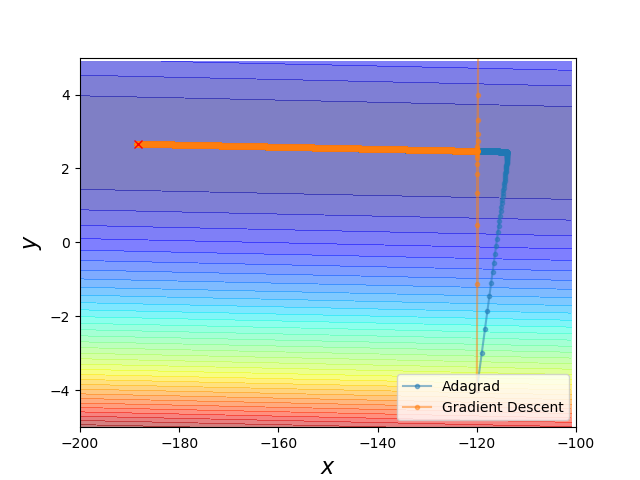
\includegraphics[width=0.3\textwidth]{w}}
			\subfigure[损失迭代]{
				\label{Fig.sub.2}
				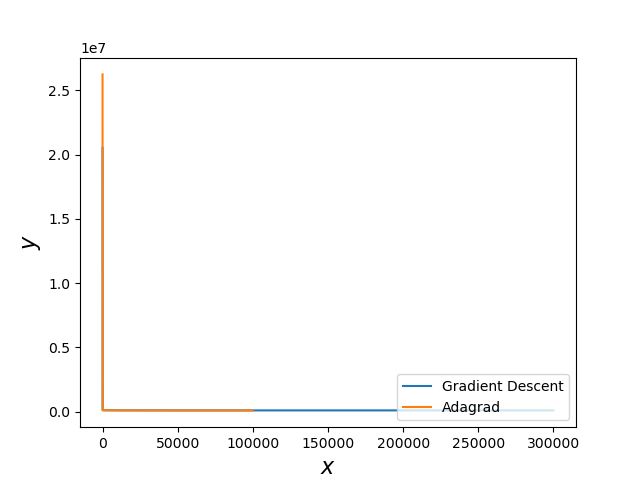
\includegraphics[width=0.3\textwidth]{loss}}
			\subfigure[回归后结果曲线]{
				\label{Fig.sub.3}
		\textbf{}		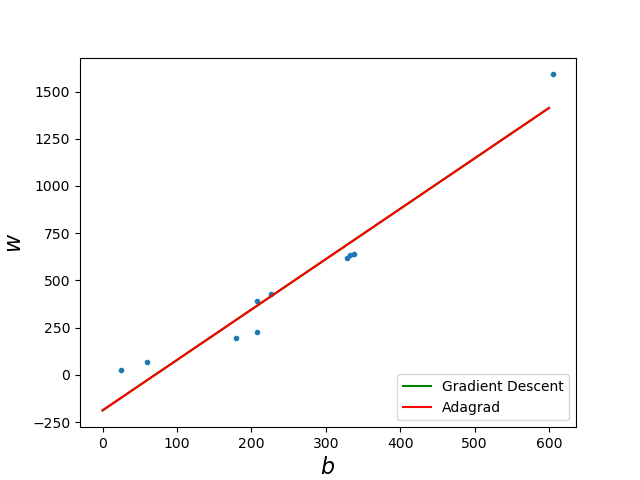
\includegraphics[width=0.3\textwidth]{line}}
			\caption{两种方式迭代后结果}
			\label{Fig.lable}
			%\caption{Visual comparison samples between the original saliency map and enhanced saliency map by centre-bias and human visual acuity.}
			\label{fig:visual_smap}
		\end{figure}		
		在图\ref{Fig.sub.1}我们还可以看到,使用Gradient Descent存在着振荡的现象,但是使用Adagrad的不存在震荡现象,但是Adagrad的梯度下降速率在后面的迭代回合几乎趋近于零,所以使用Adagrad方式能以较快速度和较好的准确性趋近于最优解,但是要想无限趋近于最优解,相比Descent Gradient需要较多的迭代回合。	
		
		
	%\subsubsection{Gradient Descent}
	%\subsubsection{Adagrad}
	%\section{分析}
\end{document}